%==================================================================%
% Author : Perez Ruiz, Alejandro                                   %
% Version: 1.0, 26/05/2011                                         %                                                                                     % Manual de la SmartHome                                           %
%==================================================================%
\documentclass[a4paper,11pt]{article}

\usepackage[latin1]{inputenc}
\usepackage{url}
\usepackage{amsfonts}
\usepackage[spanish,activeacute]{babel}
\usepackage{graphicx}

\title{User Manual to use smart home application}

\author{Alejandro P�rez \\ Dpto. Matem�ticas, Estad�stica y Computaci�n \\
		Universidad de Cantabria (Santander, Spain)}

\begin{document}

\maketitle

Before you use this manual, you should read the manual called \emph{User Manual for the creation and configuration of Smart Home models}, it is available in the next URL: 

\url{{http://www.alumnos.unican.es/apr85/documentation.html}}

This manual is divided in the different characteristics, because of this each section contains a manual for a specific characteristic. 

%%==================================================================%%
%% Author : P�rez Ruiz, Alejandro                                   %%
%% Author : S�nchez Barreiro, Pablo                                 %%
%% Version: 1.1, 14/06/2011                                         %%                                                                                    %%                                                                  %%
%% Memoria del Proyecto Fin de Carrera                              %%
%% Domain Engineering/Iteracion BaseSystem                          %%
%%==================================================================%%

\section{Heater management}
This characteristic controls the heaters, so you can change the value of the heaters through the Gateway and you can modified the degrees of the thermometer through the Simulator.

To switch on/off and change the value of all heaters, follow the next steps:
\begin{enumerate}
\item Go to the global tab for the heaters in the Gateway window.
\begin{center}
	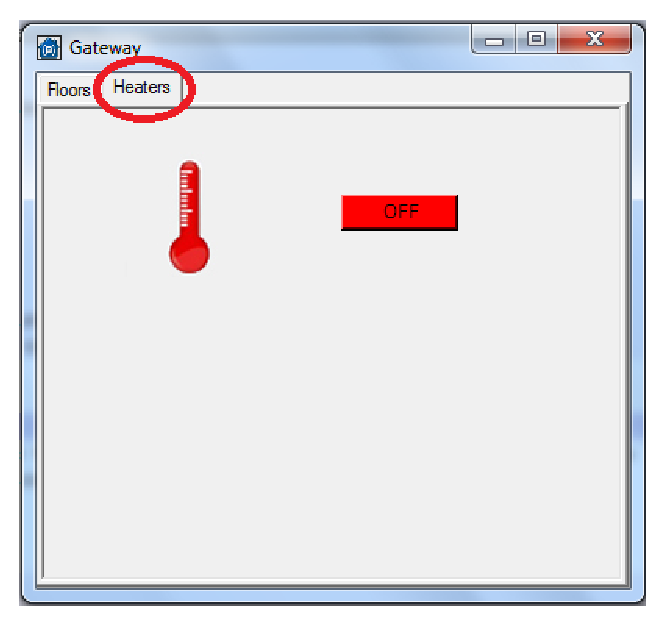
\includegraphics[width=.68\linewidth]{images/globalHeater.eps}
	\\
\vspace{1cm}
\end{center}
\item To switch on, click on the red button. Now, you can see in the Simulator window how the status of all heaters has changed.
\begin{center}
	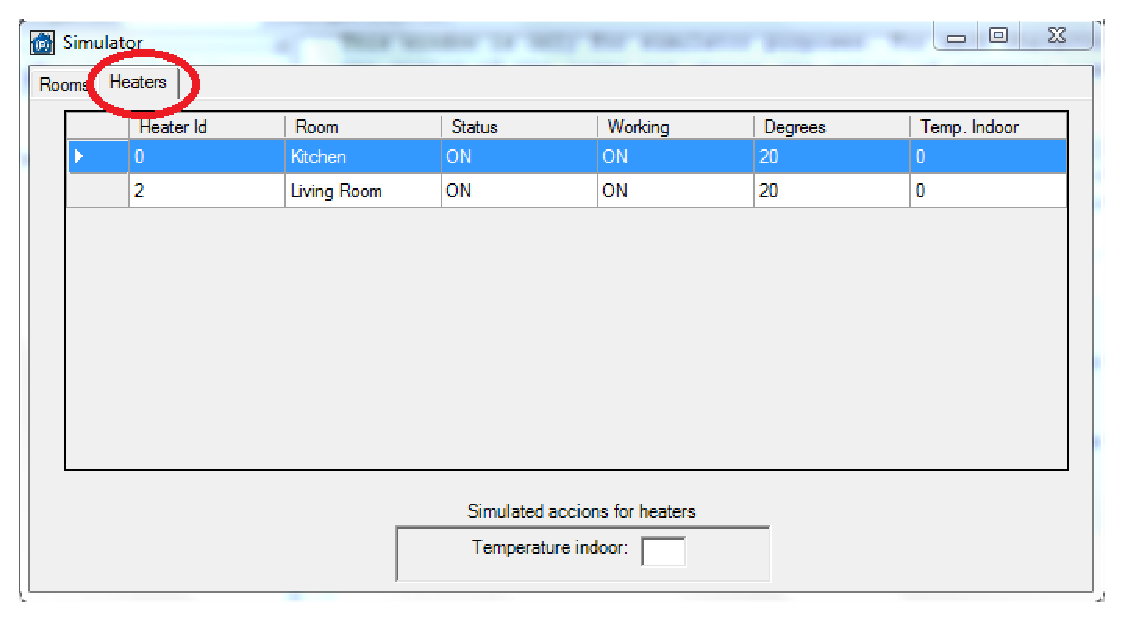
\includegraphics[width=.75\linewidth]{images/simulatorHeater.eps}
	\\
\vspace{1cm}
\end{center}
\item To change the temperature of the heaters, use the slide bar or the text box (press \emph{enter} key to confirm) to introduce a value between 0 to 40.
\begin{center}
	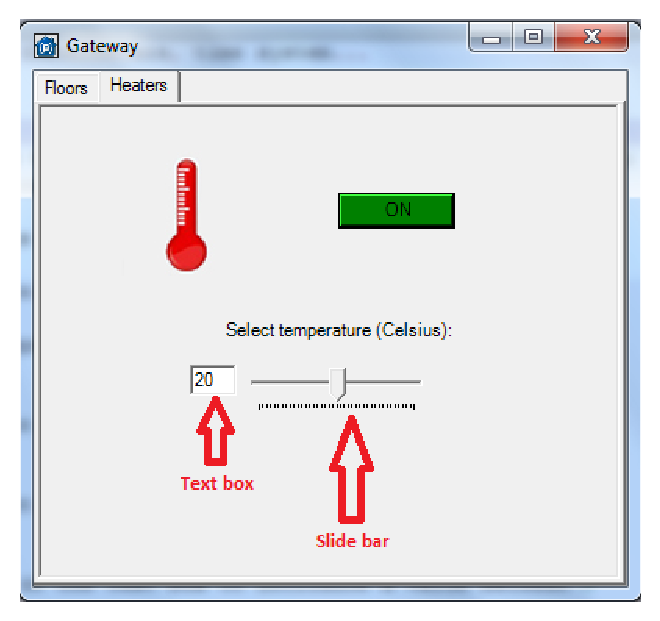
\includegraphics[width=.68\linewidth]{images/changeTemperatureHeater.eps}
	\\
\vspace{1cm}
\end{center}

\end{enumerate}
If you want to switch on/off or change the value of a specific heater, select the room where is the heater, click on the heater tab and follow the same steps to modified all heaters but in the current tab:
\begin{center}
	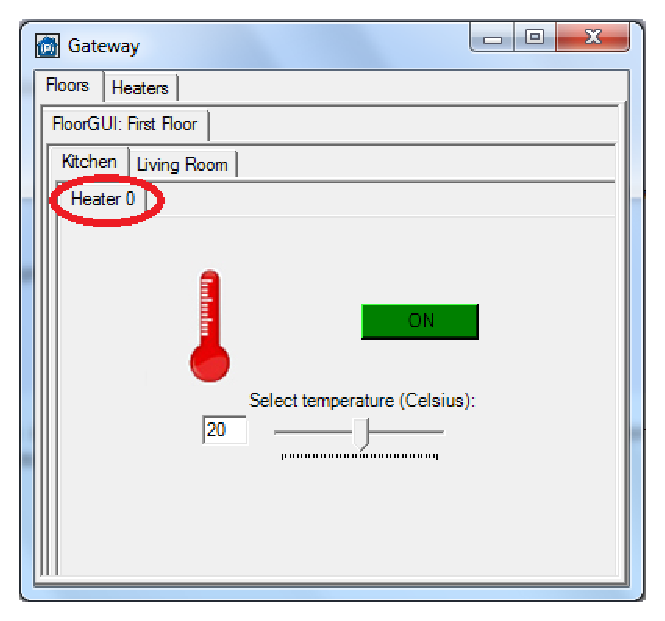
\includegraphics[width=.68\linewidth]{images/specificHeater.eps}
	\\
\vspace{1cm}
\end{center}

To change the value of a thermometer:
\begin{enumerate}
\item Go to Simulator window and select the heater tab.
\item Select a heater to change a specific thermometer. In the text box with the label \emph{Temperature indoor} introduce a value and press \emph{enter} key.
\begin{center}
	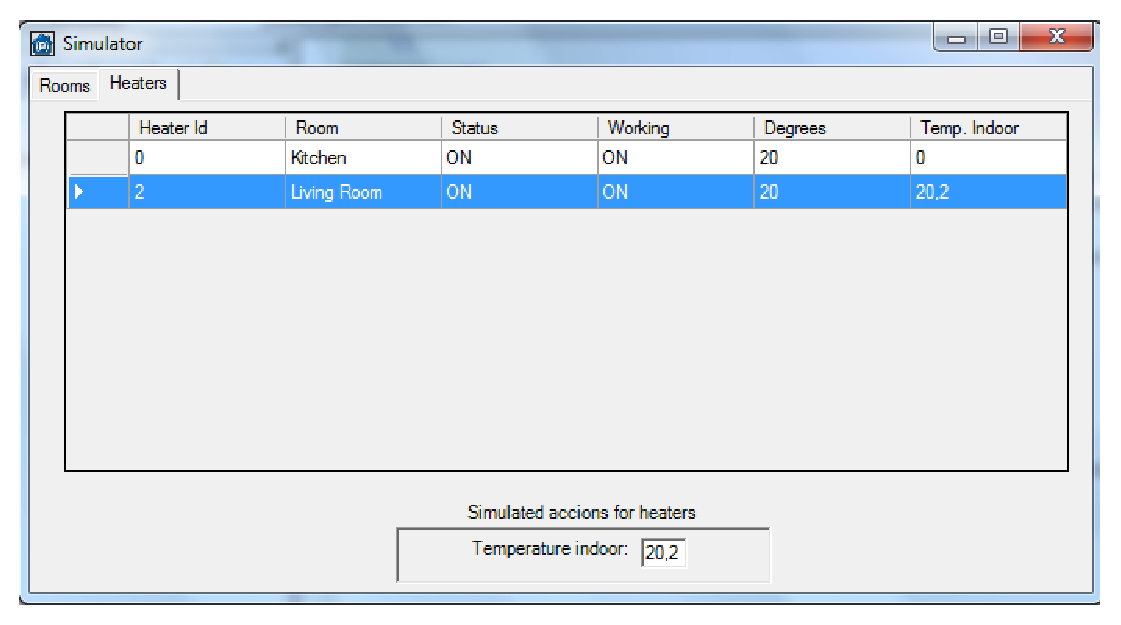
\includegraphics[width=.68\linewidth]{images/thermometerHeater.eps}
	\\
\vspace{1cm}
\end{center}
\end{enumerate}
If the temperature of a thermometer and its heater are equal, the heater will be \emph{OFF} in the \emph{Working} cell in the Simulator window, because of this, the heater won't waste energy. 

\section{Window management}
This characteristic controls the windows, so you can change the aperture of the windows through the Gateway and you can see a table with all information about windows through the Simulator.

To change the aperture of all windows, follow the next steps:
\begin{enumerate}
\item Go to the global tab for the windows in the Gateway window.
\begin{center}
	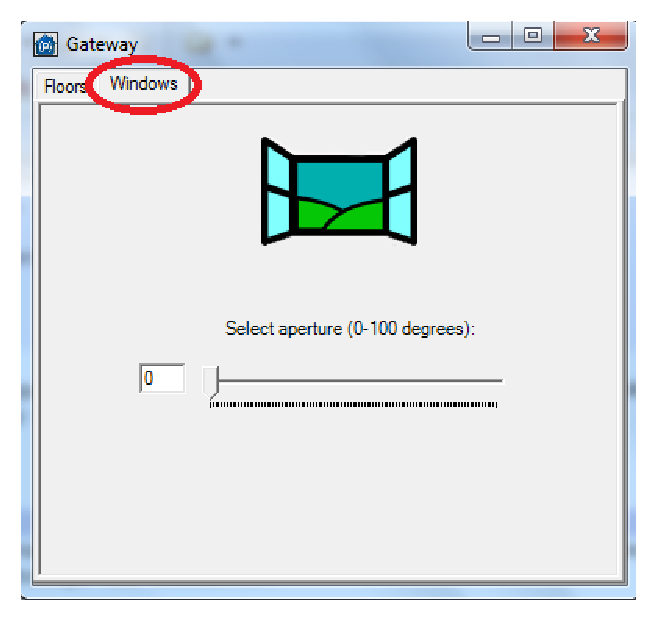
\includegraphics[width=.68\linewidth]{images/globalWindow.eps}
	\\
\vspace{1cm}
\end{center}
\item To change the aperture of the windows, use the slide bar or the text box (press \emph{enter} key to confirm) to introduce a value between 0 to 100.
\end{enumerate}
If you want to change the aperture of a specific window, select the room where is the window, click on the window tab and follow the same steps to modified all windows but in the current tab:
\begin{center}
	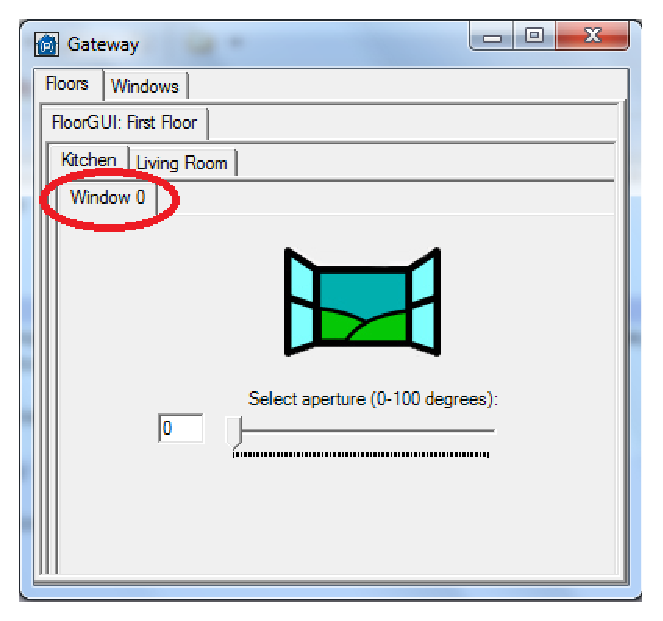
\includegraphics[width=.68\linewidth]{images/specificWindow.eps}
	\\
\vspace{1cm}
\end{center}

In the Simulator window, you have a table with the identifier, room and aperture of each window:
\begin{center}
	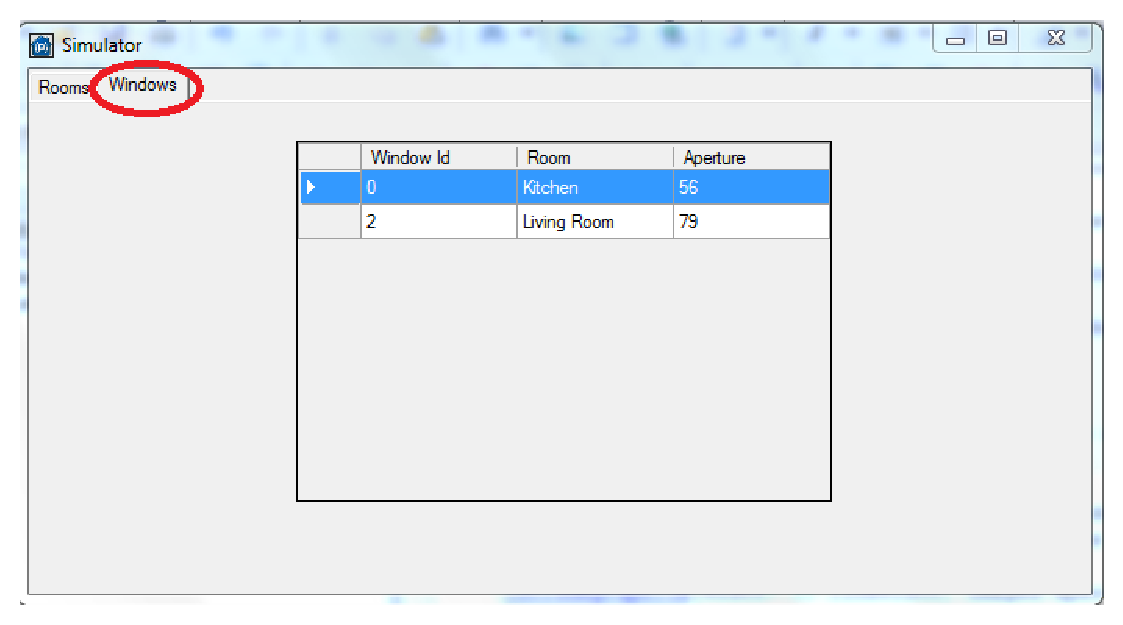
\includegraphics[width=.75\linewidth]{images/simulatorWindow.eps}
	\\
\vspace{1cm}
\end{center}

\section{Light management}
This characteristic controls the lights, so you can change the lightness of the lights through the Gateway and you can see a table with all information about lights through the Simulator.

To change the lightness of all lights, follow the next steps:
\begin{enumerate}
\item Go to the global tab for the lights in the Gateway window.

\item To change the lightness of all lights, use the slide bar or the text box (press \emph{enter} key to confirm) or predefined values to introduce a value between 0 to 100.
\begin{center}
	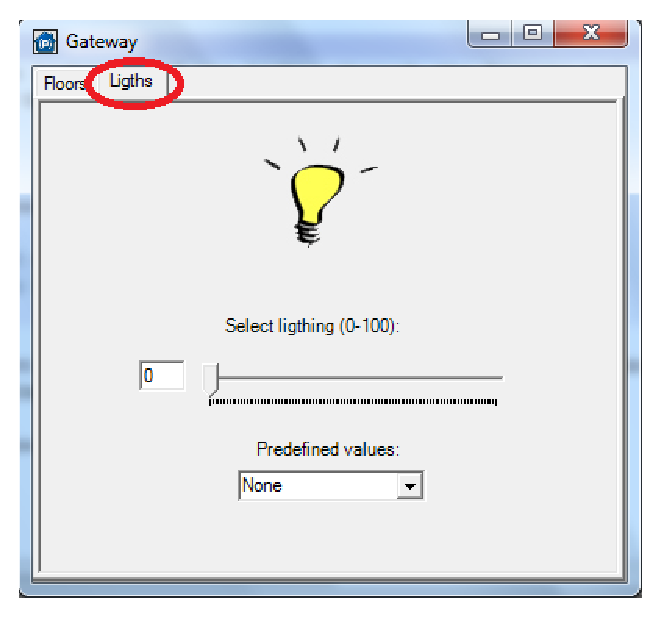
\includegraphics[width=.68\linewidth]{images/globalLight.eps}
	\\
\vspace{1cm}
\end{center}


\end{enumerate}
If you want to change the lightness of a specific light, select the room where is the light, click on the light tab and follow the same steps to modified all lights but in the current tab:
\begin{center}
	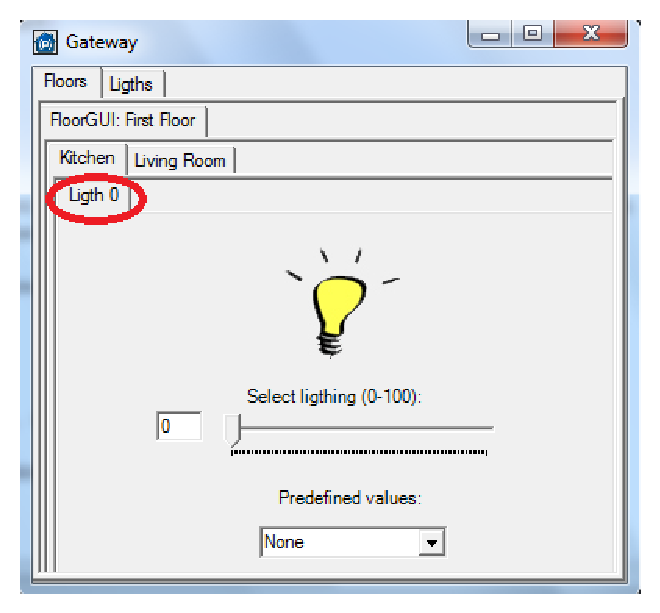
\includegraphics[width=.68\linewidth]{images/specificLight.eps}
	\\
\vspace{1cm}
\end{center}

In the Simulator window, you have a table with the identifier, room and aperture of each light:
\begin{center}
	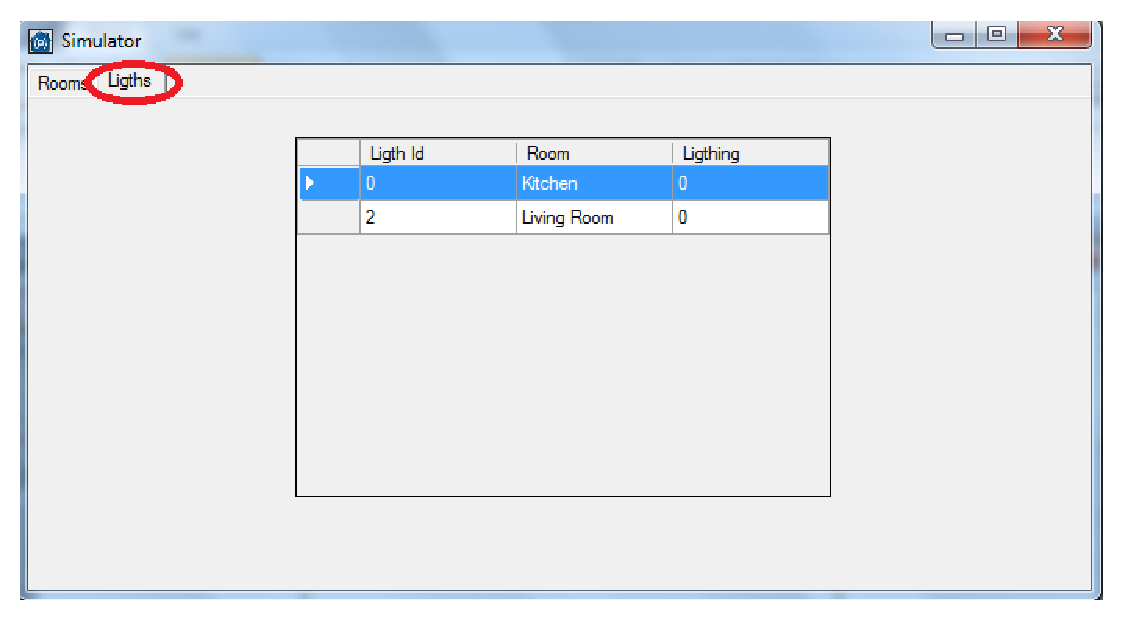
\includegraphics[width=.75\linewidth]{images/simulatorLight.eps}
	\\
\vspace{1cm}
\end{center}

\section{Blind management}
This characteristic controls the blinds, so you can change the aperture of the blinds through the Gateway and you can see a table with all information about blinds through the Simulator.

To change the aperture of all blinds, follow the next steps:
\begin{enumerate}
\item Go to the global tab for the blinds in the Gateway window.
\begin{center}
	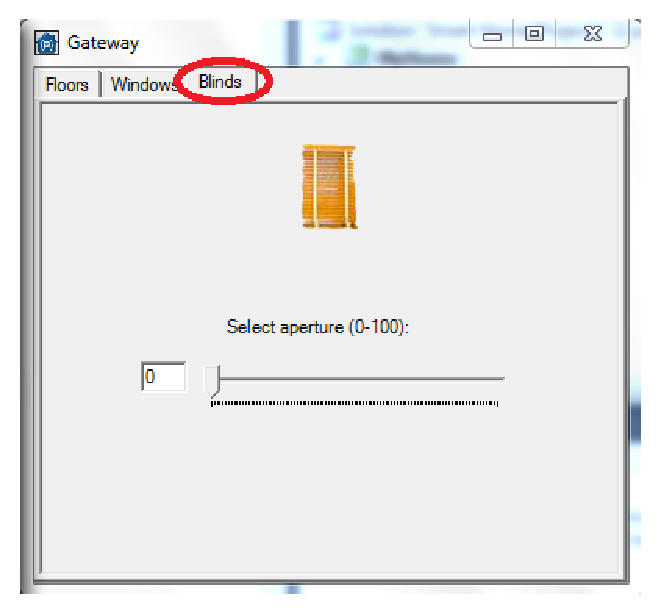
\includegraphics[width=.68\linewidth]{images/globalBlind.eps}
	\\
\vspace{1cm}
\end{center}
\item To change the aperture of the blinds, use the slide bar or the text box (press \emph{enter} key to confirm) to introduce a value between 0 to 100.
\end{enumerate}
If you want to change the aperture of a specific blind, select the room where is the blind, click on the blind tab and follow the same steps to modified all blinds but in the current tab:
\begin{center}
	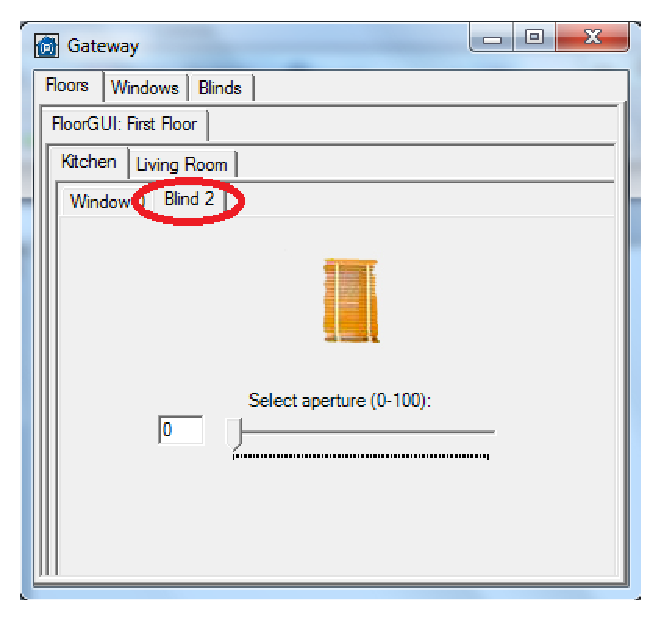
\includegraphics[width=.68\linewidth]{images/specificBlind.eps}
	\\
\vspace{1cm}
\end{center}

In the Simulator window, you have a table with the identifier, room, window and aperture of each blind:
\begin{center}
	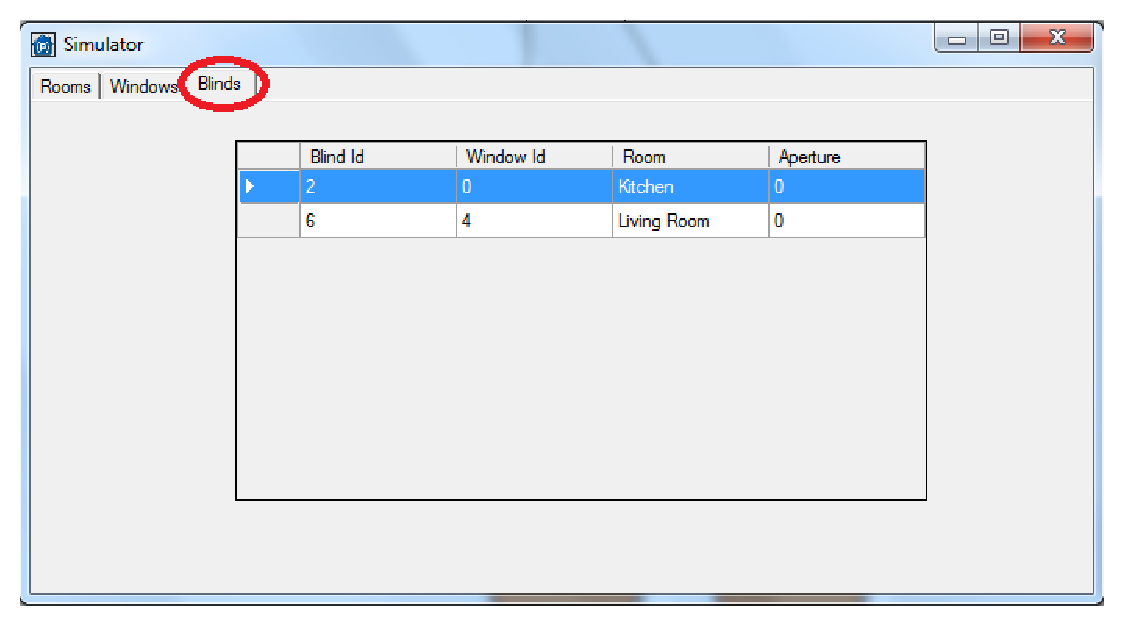
\includegraphics[width=.75\linewidth]{images/simulatorBlind.eps}
	\\
\vspace{1cm}
\end{center}

\section{Smart energy management}
This characteristic has two main functionalities:
\begin{enumerate}
\item If a window is opened when the heaters are working,this window will be closed automatically.
\item The daily schedule of each inhabitant is stored in a XML file. In the periods of the day when the house is empty, the heaters are disconnected and reconnected with enough time to reach the desired temperature when the inhabitants come back home.
\end{enumerate}
To activate this characteristic, go to the smartEnergy tab and click on the red button.
\begin{center}
	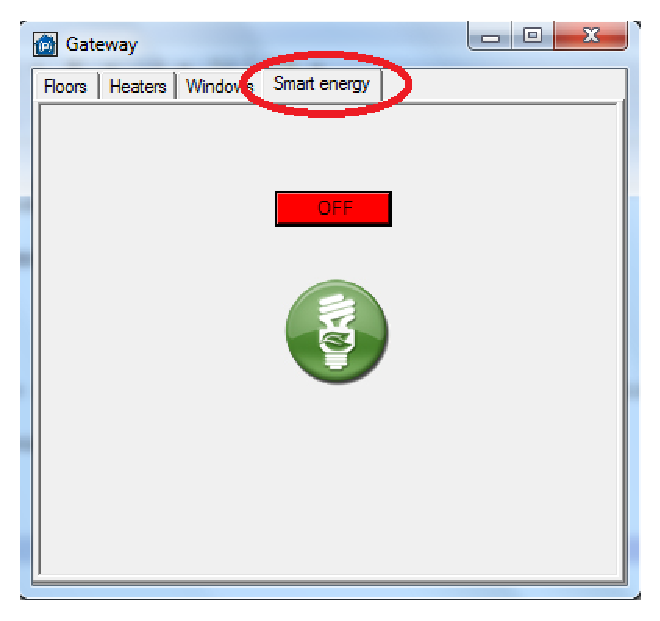
\includegraphics[width=.75\linewidth]{images/globalSmartEnergy.eps}
	\\
\vspace{1cm}
\end{center}
When this characteristic is on, you can establish the desired temperature. This temperature is used to reach an adequate temperature when the house is empty. To modify the temperature value, write your desired value and click on the button called \emph{Submit}.
\begin{center}
	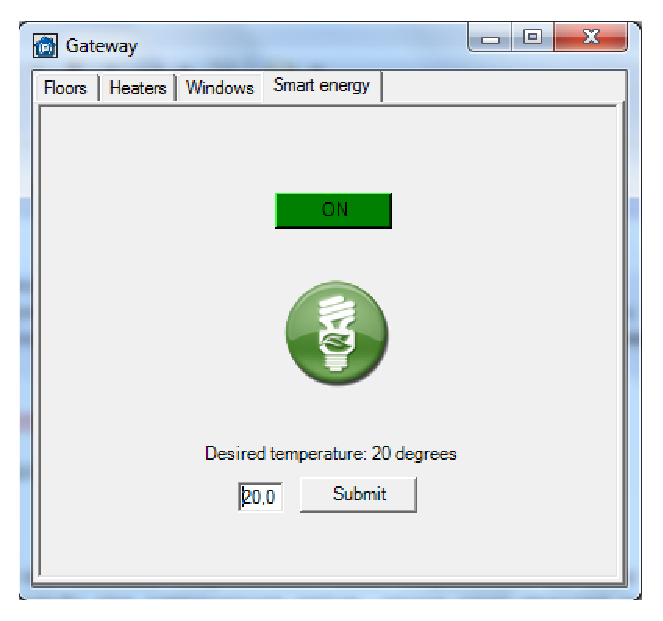
\includegraphics[width=.75\linewidth]{images/desiredTemperatureSmartEnergy.eps}
	\\
\vspace{1cm}
\end{center}
In the file \emph{timetable.xml} of your project, you can find the daily schedule of all inhabitants. If you want to change it, open it and modified tags. The tag called \emph{timetable} contains the hours where this inhabitant is outside of the house.
\begin{center}
	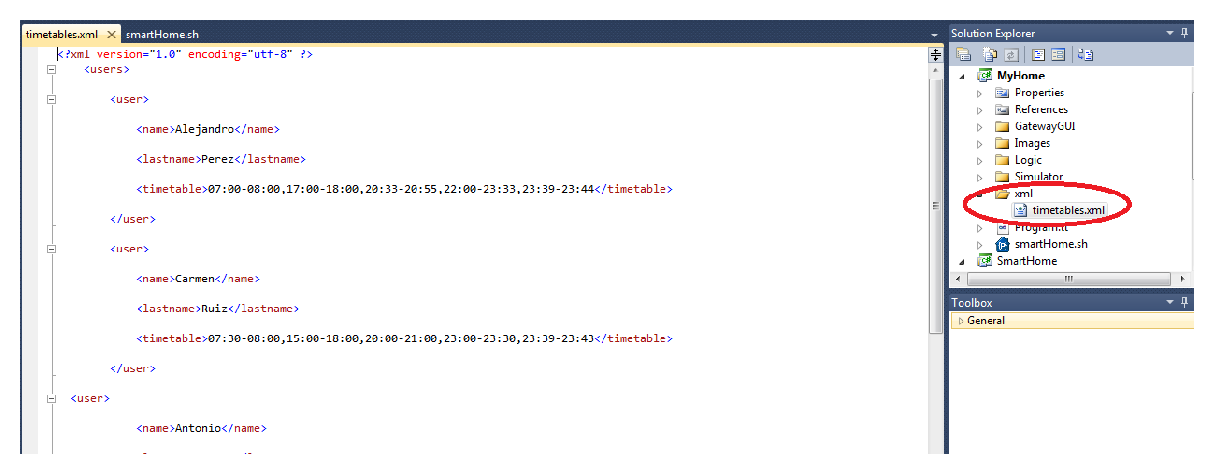
\includegraphics[width=.99\linewidth]{images/xmlSmartEnergy.eps}
	\\
\vspace{1cm}
\end{center}

In the tag called SmartEnergy in the Simulator window, you can find a list where you can see the hours when the house is empty. And you can change the current system time, so if you establish a time which nobody is in the house, all the heaters will be disconnected, unless the time is close to come back a inhabitant.
\begin{center}
	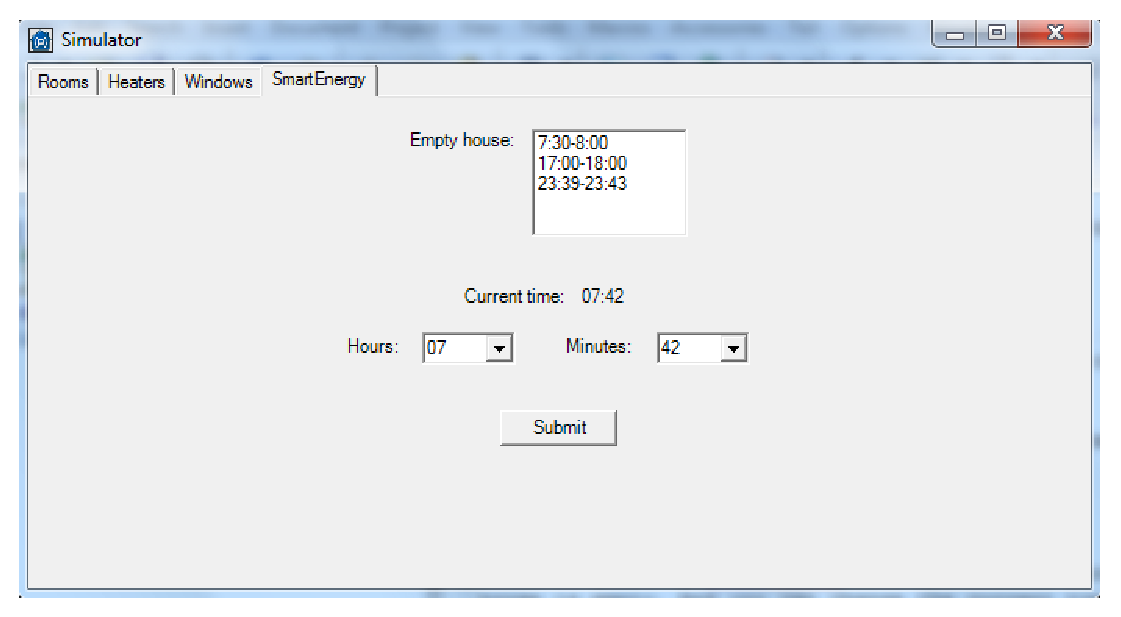
\includegraphics[width=.99\linewidth]{images/simulatorSmartEnergy.eps}
	\\
\vspace{1cm}
\end{center}


\section{Light simulation}

Lights are switched on/off in order to simulate presence. They are switched on/off using a semi random schema, in this case, the lightness of each light is modified every hour.

To activate this characteristic go to LightSimulation tab and click on the red button:
\begin{center}
	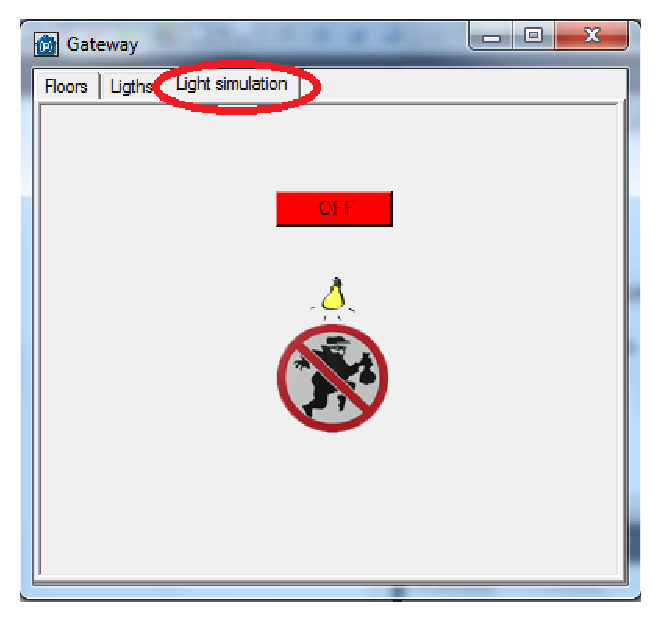
\includegraphics[width=.75\linewidth]{images/globalLightSimulation.eps}
	\\
\vspace{1cm}
\end{center}

In the tag called LightSimulation in the Simulator window, you can modified the current system time.
\begin{center}
	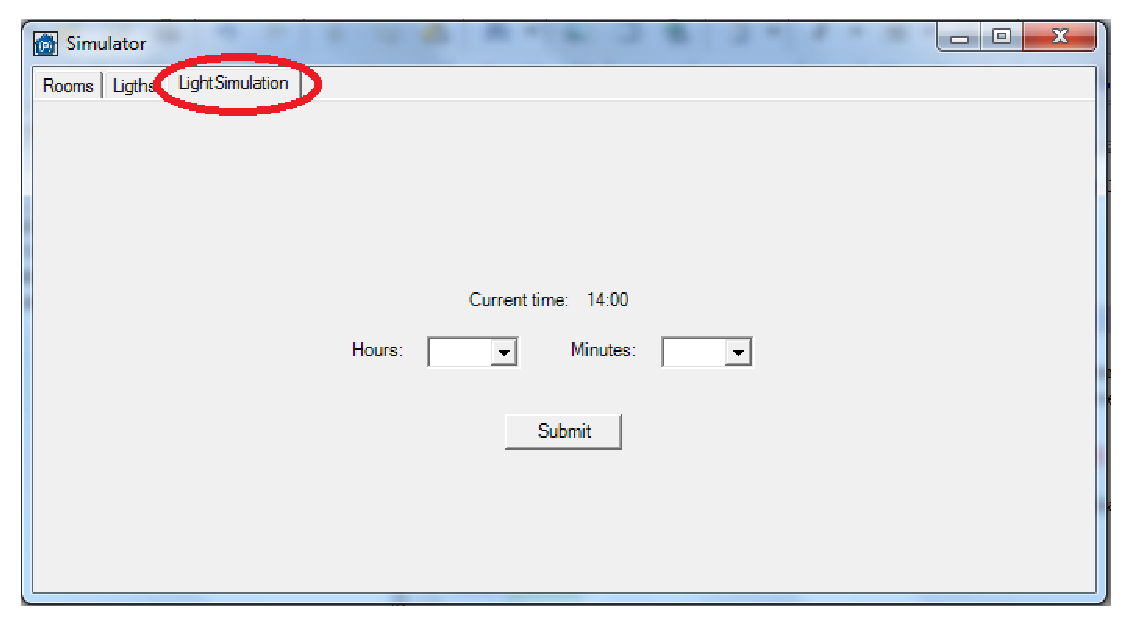
\includegraphics[width=.99\linewidth]{images/simulatorLightSimulation.eps}
	\\
\vspace{1cm}
\end{center}

\section{Blind simulation}
Blinds are automatically rolled up and down in order to simulate presence. They are rolled up and down using a semi random schema, in this case, the aperture of each blind is modified every hour.

To activate this characteristic go to BlindSimulation tab and click on the red button:
\begin{center}
	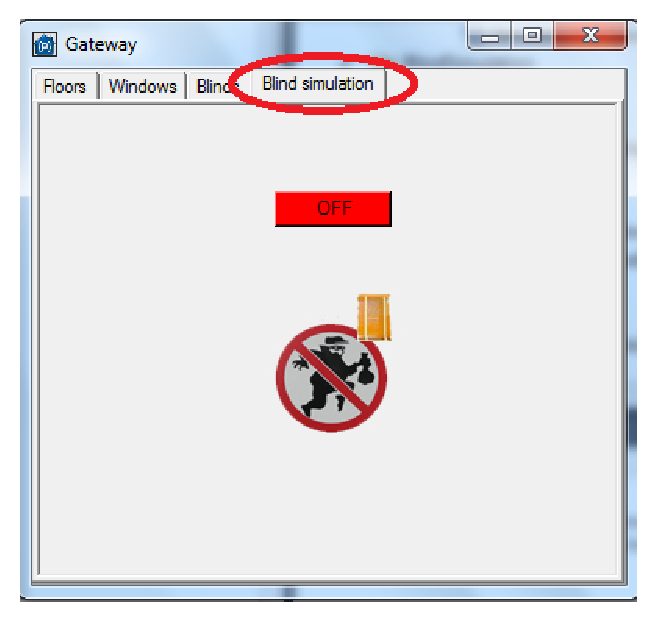
\includegraphics[width=.65\linewidth]{images/globalBlindSimulation.eps}
	\\
\vspace{1cm}
\end{center}

In the tag called BlindSimulation in the Simulator window, you can modified the current system time.
\begin{center}
	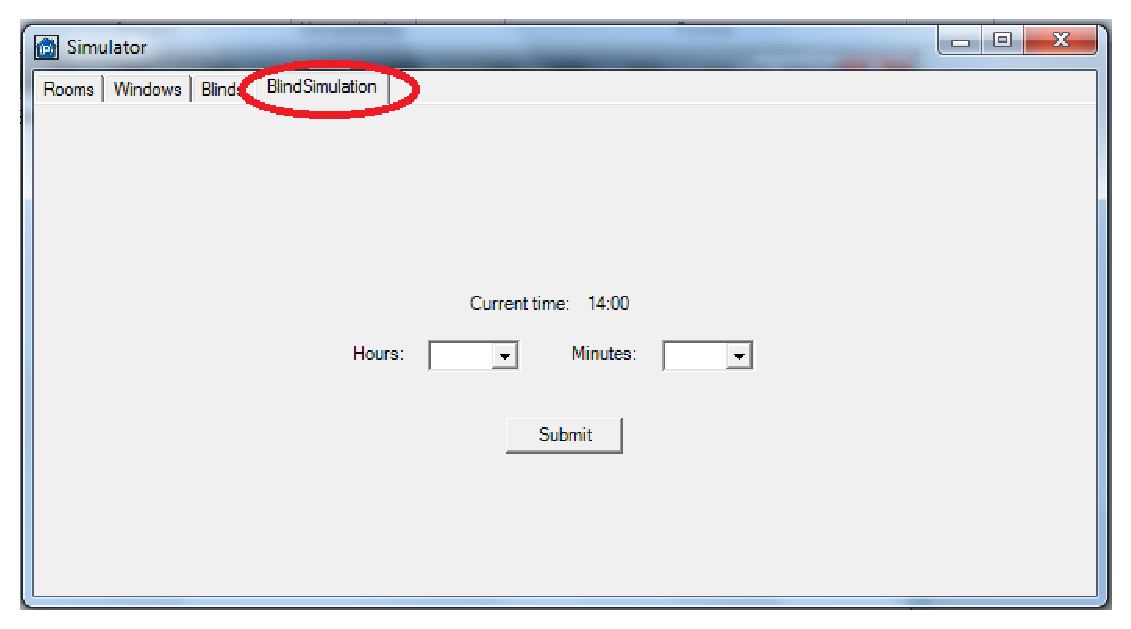
\includegraphics[width=.99\linewidth]{images/simulatorBlindSimulation.eps}
	\\
\vspace{1cm}
\end{center}

\end{document}




